\documentclass[a4paper,ngerman,twoside]{scrartcl}

\usepackage[utf8]{inputenc}
\usepackage[ngerman]{babel}
\usepackage{amsmath,amsthm,amssymb,amscd,color,graphicx,environ,mathtools}
\usepackage{framed}
\usepackage[protrusion=true,expansion=true]{microtype}
\usepackage{lmodern}
\usepackage{multicol}
\usepackage[normalem]{ulem}
\usepackage{hyperref}

\newcommand{\defeq}{\vcentcolon=}

\setlength{\unitlength}{1cm}

\setlength\parskip{\medskipamount}
\setlength\parindent{0pt}

\renewcommand*\theenumi{\alph{enumi}}
\renewcommand{\labelenumi}{\theenumi)}

\newlength{\aufgabenskip}
\setlength{\aufgabenskip}{1.4em}
\newcounter{aufgabennummer}
\newenvironment{aufgabe}[1]{
  \addtocounter{aufgabennummer}{1}
  \textbf{Aufgabe \theaufgabennummer.} \emph{#1} \par
}{\vspace{\aufgabenskip}}
\newenvironment{aufgabe*}[1]{
  \addtocounter{aufgabennummer}{1}
  \textbf{Aufgabe* \theaufgabennummer.} \emph{#1} \par
}{\vspace{\aufgabenskip}}
\newenvironment{aufgabeE}[1]{\begin{aufgabe}{#1}\begin{enumerate}}{\end{enumerate}\end{aufgabe}}

\clubpenalty=10000
\widowpenalty=10000
\displaywidowpenalty=10000

\newcommand{\NN}{\mathbb{N}}
\newcommand{\RR}{\mathbb{R}}
\DeclarePairedDelimiter{\floor}{\lfloor}{\rfloor}

\begin{document}

\thispagestyle{empty}
Institut für Mathematik \\
Universität Augsburg \\
Ingo Blechschmidt

\begin{center}
  \textbf{Pizzaseminar in Mathematik} \\
  \emph{Das Geheimnis der Zahl 5}
\end{center}
\vspace{1em}

Die \emph{Folge der Fibonacci-Zahlen} beginnt mit
\[
  f_0 \defeq 1, \quad
  f_1 \defeq 1, \quad
  f_2 \defeq 2, \quad
  f_3 \defeq 3, \quad
  f_4 \defeq 5, \quad
  f_5 \defeq 8.
\]
Für~$n \geq 1$ gilt also $f_{n+1} = f_n + f_{n-1}$. Der \emph{goldene Schnitt}
ist die Zahl~$\Phi \defeq (1+\sqrt{5})/2$.
\vspace{1em}

\begin{aufgabe}{Ein Kästchen verschwindet!}
Die beiden Figuren bestehen offensichtlich aus denselben Stücken, haben
aber unterschiedlichen Flächeninhalt! Was ist passiert?
\begin{center}
  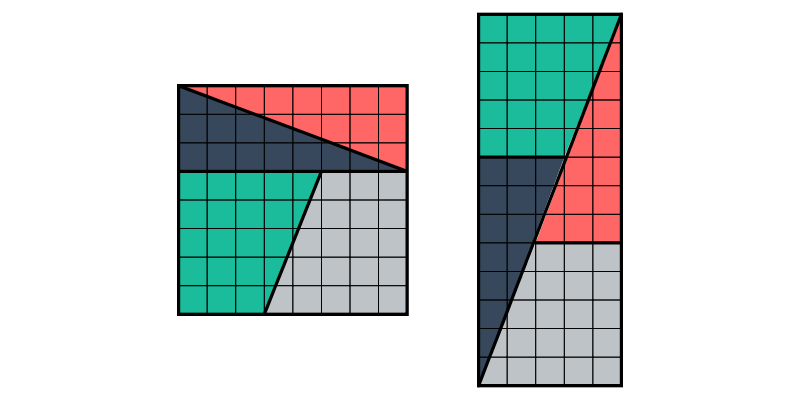
\includegraphics[scale=0.3]{ein-kaestchen-verschwindet}
\end{center}
\end{aufgabe}

\begin{aufgabe}{Die Quadrate der Fibonacci-Zahlen}
Es gilt die Identität~$f_0^2 + f_1^2 + \cdots + f_n^2 = f_n f_{n+1}$.
\begin{enumerate}
\item Führe einen Induktionsbeweis.
\item Argumentiere, wieso folgende Skizze die Behauptung auch schon beweist.
\end{enumerate}
\begin{center}
  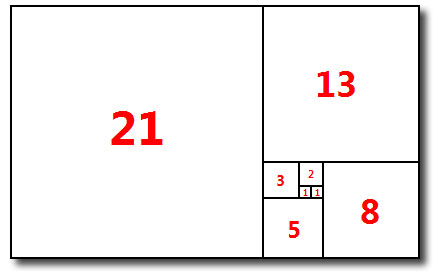
\includegraphics[scale=0.3]{fibonacci-quadrate}
\end{center}
\end{aufgabe}

\begin{aufgabe}{Von Fibonacci-Zahlen und Rechtecken}
Gegeben sei eine Reihe von~$n$ Quadraten, die ein~$(1 \times n)$-Rechteck
bilden. Wir möchten dieses Rechteck mit Monominos, also
$(1 \times 1)$-Rechtecken, sowie Dominos, $(1\times 2)$-Rechtecken, überdecken.

Zeige, dass die Anzahl von möglichen Überdeckungen des $(1 \times n)$-Rechtecks
mittels Monominos und Dominos gleich~$f_n$ ist.
\end{aufgabe}
% \url{https://www.math.hmc.edu/~benjamin/papers/DIE.pdf}

\begin{aufgabe}{Ein naiver Algorithmus für Fibonacci-Zahlen}
Eine ganz naive Methode, die~$n$-te Fibonacci-Zahl zu bestimmen, besteht
darin, die beiden Vorgänger zu bestimmen und dann zu summieren. Wie viele
Rechenschritte sind dabei notwendig, wenn man sich
Zwischenergebnisse \emph{nicht} merkt und daher viele Fibonacci-Zahlen immer wieder
berechnet?
\end{aufgabe}

\begin{aufgabe}{Fibonacci-Zahlen im Pascalschen Dreieck}
Im Pascalschen Dreieck verbergen sich die Fibonacci-Zahlen wie angedeutet.
Beweise das!
\begin{center}
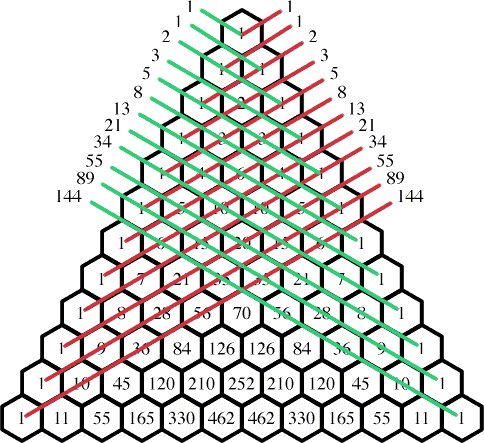
\includegraphics[scale=0.5]{pascal-fibonacci}
\end{center}
\end{aufgabe}

\begin{aufgabe}{Ein Lemma über goldene Dreiecke}
\begin{enumerate}
\item Zeige: In einem gleichschenkligen Dreieck mit den
Innenwinkeln~$72^\circ$, $36^\circ$ und~$72^\circ$ teilen die langen Seiten die
Grundseite im goldenen Schnitt.
\item Beweise damit folgende Pentagon-Dekagon-Hexagon-Identität: Seien ein
reguläres Pentagon, ein reguläres Dekagon und ein reguläres Hexagon in einem
Kreis einbeschrieben. Dann gilt für die Kantenlängen~$P$,~$D$ bzw.~$H$ die
Identität $P^2 = D^2 + H^2$.
\end{enumerate}
\end{aufgabe}

\begin{aufgabe}{Ikosaeder und Dodekaeder}
Sei einem regelmäßigen Ikosaeder ein regelmäßiges Dodekaeder einbeschrieben
(Seitenflächenmittelpunkte auf Ecken). Zeige, dass das Verhältnis der Kantenlängen
beider Objekte gleich $3:\Phi$ ist.
\end{aufgabe}

\begin{aufgabe}{Kettenbruchentwicklung des goldenen Schnitts}
\begin{enumerate}
\item Zeige: $\Phi = 1 + \frac{1}{\Phi}$. Bonuspunkte gibt es, wenn
du diese Identität allein mit der geometrischen Definition des goldenen
Schnitts nachweist: Die Gesamtstrecke verhält sich zur größeren Teilstrecke
wie die größere Teilstrecke zu kleineren.
\item Folgere:
\[ \Phi = 1 + \frac{1}{1 + \dfrac{1}{1 + \frac{1}{\ddots}}}. \]
\item Zeige: Die sukzessiven Approximationen des goldenen Schnitts, die sich
durch Abschneidung der Kettenbruchentwicklung ergeben, sind von der
Form~$f_{n+1}/f_n$.
\end{enumerate}
\end{aufgabe}

\begin{aufgabe}{Ableitung vs. Umkehrfunktion}
Finde eine bijektive differenzierbare Funktion~$\RR^+ \to \RR^+$, deren
Ableitung gleich ihrer Umkehrfunktion ist.

\emph{Tipp:} Versuche es mit dem Ansatz~$x \mapsto x^a$.
\end{aufgabe}

\begin{aufgabe}{Kettenbruckentwicklung durch den euklidischen Algorithmus}
Sei~$x$ eine nichtnegative reelle Zahl. Der euklidische Algorithmus produziere
folgende Gleichungen:
\begin{align*}
  x &= a_0 \cdot \sbox0{$r_0$}\makebox[\wd0][l]{$1$} + r_0 \\
  1 &= a_1 \cdot r_0 + r_1 \\
  r_0 &= a_2 \cdot r_1 + r_2 \\
  r_1 &= a_3 \cdot r_2 + r_3 \\
  r_2 &= a_4 \cdot r_3 + r_4
\end{align*}
Und so weiter. Die Zahlen~$a_n$ und~$r_n$ sind also nichtnegative ganze Zahlen
und die Reste~$r_n$ sind jeweils kleiner als der zweite Faktor des
nebenstehenden Produkts. Zeige:
\[ x = a_0 + \dfrac{1}{a_1 + \dfrac{1}{a_2 + \dfrac{1}{\ddots}}}. \]
\end{aufgabe}

\begin{aufgabe}{Beispiele für Kettenbruchentwicklungen}
\begin{enumerate}
\item Bestätige, dass~$\sqrt{2} = [1; 2, 2, \ldots]$.
\item Bestätige, dass~$\sqrt{3} = [1; 1, 2, 1, 2, 1, 2, \ldots]$.
\item Was ist die Kettenbruchentwicklung von~$\sqrt{5}$?
\item Mach dir nur klar: Jede reelle Zahl ist Lösung irgendeiner quadratischen
Gleichung.
\item Zeige: Jede Zahl mit periodischer Kettenbruchentwicklung ist Lösung einer
gewissen quadratischen Gleichung \emph{mit rationalen Koeffizienten}.
\end{enumerate}
\end{aufgabe}

\begin{aufgabe*}{Rekursionsformel für die Kettenbruchapproximationen}\label{rec}
Sei ein unendlicher Kettenbruch der Form
\[ [c_0;c_1,c_2,\ldots] = c_0 + \dfrac{1}{c_1 + \dfrac{1}{c_2 + \dfrac{1}{\ddots}}} \]
gegeben. Wenn man diesen sukzessive abschneidet, erhält man die Approximationen
\[ c_0, \qquad
  c_0 + \dfrac{1}{c_1} = \frac{c_0c_1 + 1}{c_1}, \qquad
  c_0 + \dfrac{1}{c_1 + \dfrac{1}{c_2}} = \frac{c_0c_1c_2 + c_0 +
  c_2}{c_1c_2+1}
\]
und so weiter. Wir definieren induktiv Folgen~$A_{-1},A_0,\ldots$
und~$B_{-1},B_0,\ldots$:
\begin{align*}
  A_{-1} &= 1 & B_{-1} &= 0 \\
  A_0 &= c_0 & B_0 &= 1 \\
  A_{n+1} &= c_{n+1} A_n + A_{n-1} & B_{n+1} &= c_{n+1} B_n + B_{n-1}
\end{align*}
Zeige für alle~$n \geq 0$: Der Bruch, der sich durch Abschneidung nach
Stelle~$n$ ergibt, ist~$A_n/B_n$.

\emph{Tipp:} Versuche einen Induktionsbeweis. Verwende im Induktionsschritt die
zentrale Einsicht, dass der Kettenbruch~$[c_0;c_1,\ldots,c_n,c_{n+1}]$ gleich
dem um ein Glied kürzeren Kettenbruch~$[c_0;c_1,\ldots,c_n+1/c_{n+1}]$ ist.
\end{aufgabe*}

\vfill
\begin{center}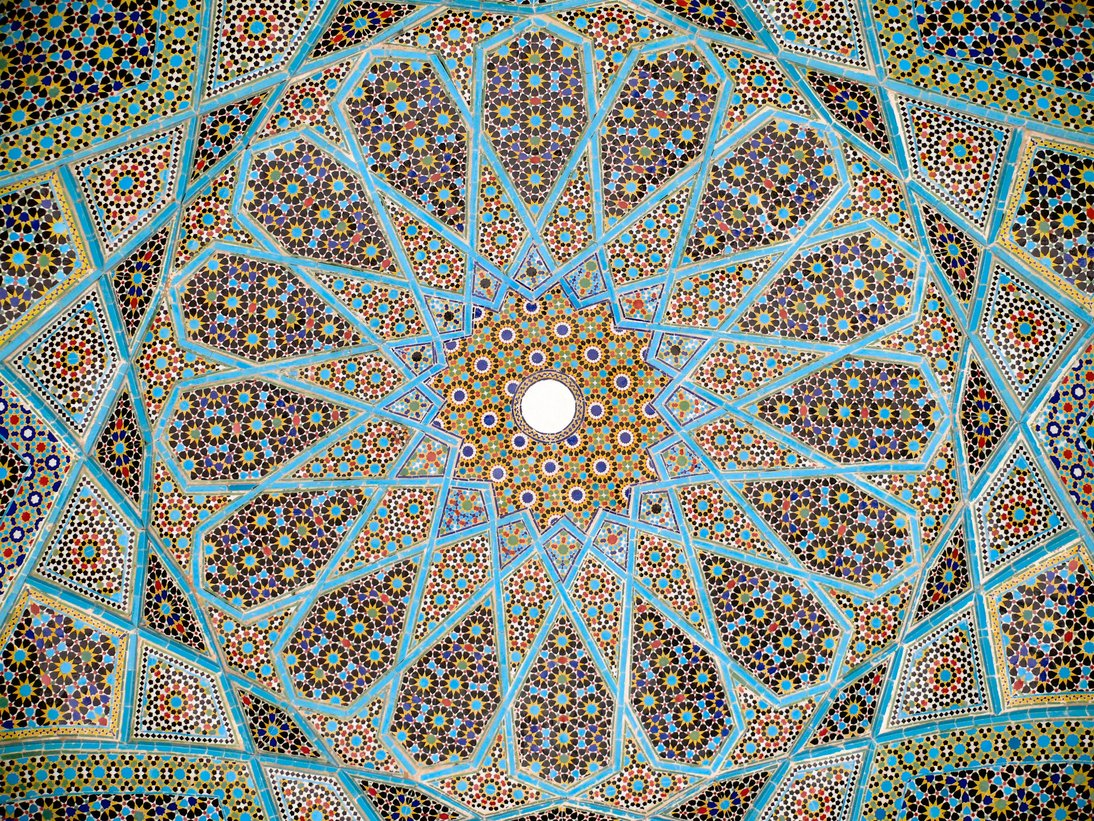
\includegraphics[width=0.60\textwidth]{hafez-tomb}\end{center}

\begin{aufgabe}{Unkürzbarkeit der Kettenbruchapproximationen}
Wie in Aufgabe~\ref{rec} schreiben wir~"`$A_n/B_n$"' für den Bruch, der sich
ergibt, wenn man die Kettenbruchentwicklung einer gegebenen Zahl abschneidet.
In dieser Aufgabe möchten wir zeigen, dass dieser Bruch stets schon gekürzt
ist.
\begin{enumerate}
\item Seien~$a$ und~$b$ zwei ganze Zahlen. Wieso sind~$a$ und~$b$ zueinander
teilerfremd, wenn es weitere ganze Zahlen~$p$ und~$q$ mit~$1 = pa + qb$ gibt?
\item Zeige für alle~$n \geq 0$: $A_{n+1} B_n - B_{n+1} A_n = (-1)^n$.
\item Ziehe das Fazit.
\end{enumerate}
\end{aufgabe}

\begin{aufgabe*}{Conways Armee}
Ein unendlich ausgedehntes Damebrett sei in zwei Hälften zerteilt. Im unteren
Teil darf man beliebig viele Damesteine platzieren. Ziel des Spiels ist es,
einen Damestein möglichst hoch in das obere Spielfeld zu
bringen. Dabei darf nur folgender Spielzug angewendet werden: Ein Stein
darf einen (horizontal oder vertikal) benachbarten Stein überspringen, wenn das
Zielfeld unbesetzt ist. Der übersprungene Stein wird dann aus dem Spiel
entfernt.
\begin{enumerate}
\item Überzeuge dich davon, dass man, um Höhe~1, 2, 3 bzw. 4 über der
Trennlinie zu erreichen, mit~2, 4, 8 bzw. \sout{16} 20 Steinen beginnen muss.
\item Zeige, dass Höhe~5 mit keiner endlichen Anzahl von Steinen erreichbar
ist.

\emph{Tipp:} Hier muss man auf geeignete Art und Weise eine von der
Feldbesetzung abhängige Größe definieren, die bei jedem Zug abnimmt. Man könnte
diese Größe zum Beispiel \emph{Energie} nennen. Dann kann man nachrechnen: Die
Energie von beliebig vielen Spielsteinen in der unteren Bretthälfte ist kleiner
als die Energie von auch nur einem einzigen Stein in Höhe~5. Eine mögliche
Definition für die Energie, die diese Anforderungen erfüllt, besteht darin, für
jeden vorhandenen Spielstein die Zahl~$(1/\Phi)^d$ aufzusummieren, wobei~$d$
die \emph{Manhattan-Entfernung} des Spielsteins zu einem beliebig ausgemachten
Ursprungsstein ist. Details findest du im Internet.
\end{enumerate}
\end{aufgabe*}

\vfill
\begin{center}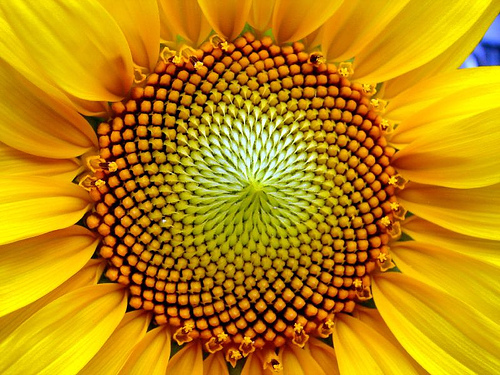
\includegraphics[width=0.45\textwidth]{sonnenblume}\end{center}

\begin{aufgabe*}{Verschoben aufsummierte Fibonacci-Zahlen}
In dieser Aufgabe betrachten wir die "`verschoben aufgeschriebenen"'
Fibonacci-Zahlen:
\begin{align*}
&0{,}1 \\
&0{,}01 \\
&0{,}002 \\
&0{,}0003 \\
&0{,}00005 \\
&0{,}000008 \\
&0{,}0000013
\end{align*}
Setzt man dieses Muster fort und summiert über alle Zeilen, so erhält man als
Summe exakt den Wert~$10/89$. Wieso?

\emph{Tipp:} Informierere dich über \emph{erzeugende Funktionen}, zum Beispiel
in dem tollen Buch \emph{Generatingfunctionology} von Herbert Wilf (auf der
Seite des Autors zu finden).
\end{aufgabe*}

\begin{aufgabe*}{Eine Zahl mit besonderer Dezimalbruchentwicklung}
Es gilt:
\[ \frac{1}{998999} =
  0{,}000\,001\,001\,002\,003\,005\,008\,013\,021\ldots. \]
\begin{enumerate}
\item Was ist daran besonders?
\item Inwiefern setzt sich das Muster auch nach~$987$ fort?
\item Erkläre das Phänomen.
\end{enumerate}
\end{aufgabe*}

\vfill
\begin{center}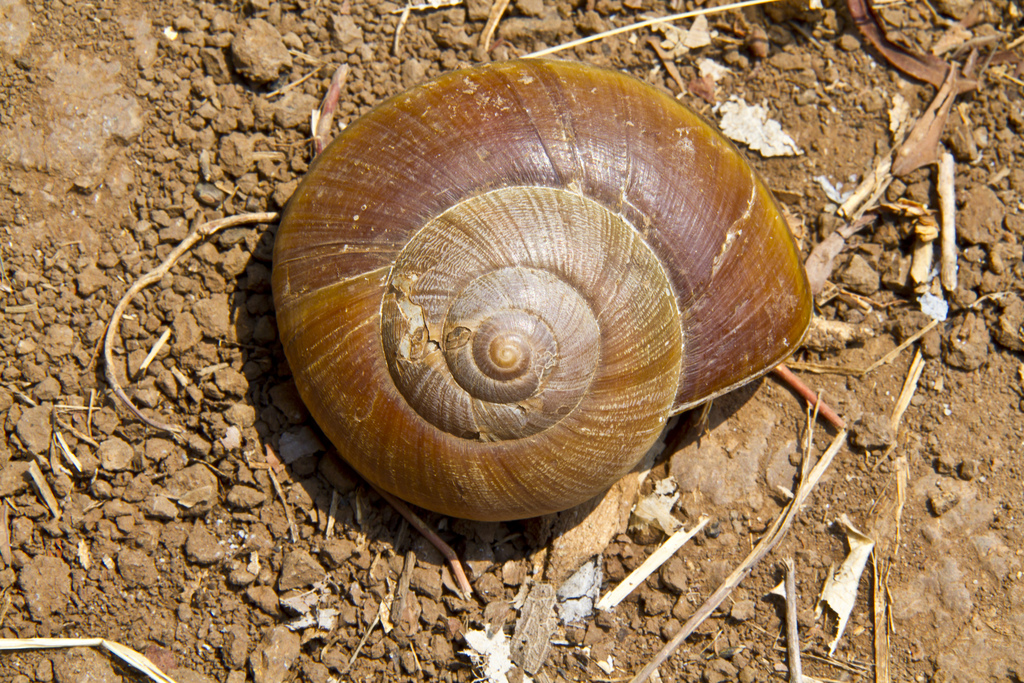
\includegraphics[width=0.73\textwidth]{goldene-spirale-8}\end{center}

\begin{aufgabe}{Spiel und Spaß mit 10-adischen Zahlen}
Bei den gewöhnlichen reellen Zahlen stehen in ihrer Dezimalschreibweise vor dem
Komma nur endlich viele Ziffern, hinter dem Komma aber gelegentlich unendlich
viele Ziffern. Bei den~$10$-adischen Zahlen ist es genau umgekehrt: Vor dem
Komma dürfen unendlich viele Ziffern stehen, hinter dem Komma dagegen nur
endlich viele. Die Rechenverfahren zur Addition, Subtraktion und
Multiplikation, wie man sie aus der Schule kennt, funktionieren weitestgehend
unverändert. Die Division wird etwas komplizierter.
\begin{enumerate}
\item Vollziehe folgende Rechnung nach:
$\ldots 13562 + \ldots 90081 = \ldots 03643$.
\item Was ist $\ldots 99999 + 1$? Dabei ist~$1 = \ldots 00001$.
\item Was ist~$-123$?
\item Finde eine~$10$-adische Zahl~$x$ -- weder Null noch Eins -- mit~$x^2 = x$.
\item Überlege dir (oder schlage nach), wie in den 10-adischen Zahlen die
Division funktioniert. Die Division durch 3, 7, 9 und alle weiteren zu~10
teilerfremden ganzen Zahlen geht übrigens \emph{stets ohne Komma auf}.
\item Gibt es in den~$10$-adischen Zahlen einer Zahl~$x$ mit der
Eigenschaft~$x = 1 + 1/x$, oder äquivalent~$x^2 = x + 1$?
\item Wie sieht es in den~$11$-adischen Zahlen aus? (Schwer ohne umfangreiche
Tipps.)
\end{enumerate}
{\scriptsize
\emph{Bemerkung:} Die Gleichung in Teilaufgabe~d) kann man zu~$x \cdot (x-1) =
0$ umstellen. In den~$10$-adischen Zahlen kann also ein Produkt Null sein, ohne
dass einer der Faktoren Null ist. Wegen dieser schlechten Eigenschaft werden
die~$10$-adischen Zahlen kaum verwendet. \emph{Allerdings:} Verwendet man als
Basis nicht~$10$, sondern eine Primzahl, so gibt es dieses Problem nicht.
Die~$2$-adischen Zahlen werden gelegentlich in der Informatik und
die~$p$-adischen Zahlen, wobei~$p$ irgendeine Primzahl ist, überall in der
Zahlentheorie verwendet. Dort gibt es beispielsweise folgendes mächtiges
"`lokal-zu-global"' Prinzip: Eine Gleichung einer bestimmten Art hat genau dann
eine Lösung in~$\mathbb{Z}$, wenn sie eine Lösung in~$\mathbb{R}$ und jeweils
eine Lösung in allen~$p$-adischen Zahlen hat.\par}
\end{aufgabe}

\end{document}

Eine ganz tolle Quelle:
http://www.math.brown.edu/~jhs/frintonlinechapters.pdf

Auch gut:
http://www.math.jacobs-university.de/timorin/PM/continued_fractions.pdf
http://www.millersville.edu/~bikenaga/number-theory/approximation-by-rationals/approximation-by-rationals.html
